\documentclass[twocolumn, 10pt]{article}
\usepackage[utf8]{inputenc}
\usepackage[T1]{fontenc}
\usepackage{geometry}
\geometry{a4paper, margin=0.75in}
\usepackage{graphicx}
\usepackage{amsmath}
\usepackage{amssymb}
\usepackage{booktabs}
\usepackage{hyperref}
\usepackage{enumitem}
\usepackage{caption}
\usepackage{tabularx}
\usepackage{booktabs}
\usepackage{tabularray}
\usepackage{tabularx}
\usepackage{booktabs}
\usepackage{seqsplit}
\usepackage{makecell}
\usepackage{setspace}
\usepackage{titlesec}
\usepackage{float}
\usepackage{colortbl}
\usepackage{xcolor}
\usepackage{listings}
\usepackage{fancyvrb}
\usepackage[most]{tcolorbox}
\tcbuselibrary{listings}

\lstset{
    language=Python,
    basicstyle=\small\ttfamily,
    breaklines=true,
    columns=flexible,
    numbers=none,
    keywordstyle=\color{blue},
    commentstyle=\color{green!40!black},
    stringstyle=\color{red!60!black},
    morekeywords={Alice,Bob,Carol,Dave,Alice:,Bob:,Carol:,Dave:,All,Derived,AES-256,key:,Decrypted},
    emph={K_AB,K_CD,g^abcd,pow,p,g^ab,g^cd},
    emphstyle=\color{blue},
    frame=single,
    tabsize=2
}

% --- Code block style (mycode) ---
\newtcblisting{mycode}[1][Python]{
    breakable,
    colback=gray!5,
    colframe=gray!50,
    arc=0pt,
    boxrule=0.5pt,
    listing only,
    listing options={
        language=#1,
        numbers=none,
        showstringspaces=false,
        breaklines=true,
        basicstyle=\small\ttfamily,
        keywordstyle=\color{blue},
        commentstyle=\color{green!40!black},
        stringstyle=\color{red!60!black}
    },
    left=5pt, right=5pt, top=5pt, bottom=5pt
}

% --- Inline code box (\codebox) ---
\newtcbox{\codebox}{on line,
    arc=2pt,
    boxsep=0pt,
    left=3pt, right=3pt,
    top=2.5pt, bottom=2.5pt,
    colback=gray!20,
    colframe=gray!120,
    boxrule=0.5pt,
    size=minimal,
    fontupper=\ttfamily\small
}

\titlespacing*{\section}
{0pt}{1.0ex plus .2ex minus .2ex}{0.3ex plus .1ex}
\titlespacing*{\subsection}
{0pt}{1ex plus .2ex minus .2ex}{0.3ex plus .1ex}
\titlespacing*{\subsubsection}
{0pt}{0.5ex plus .1ex minus .1ex}{0pt}

\setstretch{0.93}
\setlength{\belowcaptionskip}{-10pt}
\setlength{\textfloatsep}{10pt plus 1.0pt minus 2.0pt}

\begin{document}

% --- Header ---
\begin{center}
    {\Large \textbf{COMP232 Cyber Security --- Assignment 2}} \\[0.3em]
    \textbf{COMP232} \quad | \quad \textbf{\today} \\[0.4em]
    {\small \href{mailto:sgzjia24@liverpool.ac.uk}{Zhibin Jiang}}
    \vspace{0.2em}
    \hrule height 0.8pt
\end{center}

% ============================================================
\section{Comparison of Message Authentication Methods}
% ============================================================

The three methods below are compared across \textbf{integrity}, \textbf{authentication}, and \textbf{non-repudiation}, as studied in Labs 5 and 6.

% --------------------------------
\subsection{Hash Functions (SHA-256)}
% --------------------------------

\textbf{Purpose \& assumptions.} Maps an arbitrary message to a fixed 256-bit digest. Used solely for \emph{integrity checking}: any bit-flip in the input changes the digest entirely. Assumes collision resistance and pre-image resistance; no key is required.

\textbf{Security properties.}
\begin{itemize}[leftmargin=*, itemsep=0pt, topsep=1pt]
    \item \textbf{Integrity:} Receiver recomputes \codebox{SHA256(m)} and compares with the received digest.
    \item \textbf{Authentication:} \emph{Not provided} --- anyone can compute the hash; no proof of origin.
    \item \textbf{Non-repudiation:} \emph{Not provided} --- no secret links the digest to a specific sender.
\end{itemize}

\textbf{Pros:} Fast, keyless, compact output (32 bytes).\\
\textbf{Cons:} Integrity only; must be combined with a keyed scheme for authentication.

% --------------------------------
\subsection{Digital Signatures (RSA/DSA)}
% --------------------------------

\textbf{Purpose \& assumptions.} As practised in Lab 5, the sender computes $h{=}H(m)$ and signs it with their \emph{private key}: $\sigma = \text{RSA}_\mathit{priv}(h)$. The receiver verifies using the sender's \emph{public key}. Assumes hardness of integer factorisation (RSA) and collision resistance of the hash; requires a trusted public key.

\textbf{Security properties.}
\begin{itemize}[leftmargin=*, itemsep=0pt, topsep=1pt]
    \item \textbf{Integrity:} Signature verification fails if $m$ is altered.
    \item \textbf{Authentication:} Only the private-key holder can produce a valid $\sigma$.
    \item \textbf{Non-repudiation:} Any third party can verify $\sigma$ with the public key; the sender cannot deny signing.
\end{itemize}

\textbf{Pros:} Provides all three properties; public verification needs no shared secret.\\
\textbf{Cons:} Computationally expensive; depends on PKI for key distribution.

% --------------------------------
\subsection{HMAC-SHA256}
% --------------------------------

\textbf{Purpose \& assumptions.} As studied in Lab 6, HMAC mixes a shared secret key $K$ with the message through two nested hash calls, producing a 256-bit tag. Assumes SHA-256 pseudo-randomness and that both parties have already established $K$ securely (e.g., via Diffie-Hellman from Lab 4).

\textbf{Security properties.}
\begin{itemize}[leftmargin=*, itemsep=0pt, topsep=1pt]
    \item \textbf{Integrity:} Receiver recomputes \codebox{HMAC(K,m)} and checks it matches the tag.
    \item \textbf{Authentication:} Only parties holding $K$ can generate or verify the tag.
    \item \textbf{Non-repudiation:} \emph{Not provided} --- since $K$ is shared, either party could have produced the tag; no third-party proof is possible.
\end{itemize}

\textbf{Pros:} Fast; stronger than a plain keyed hash (resistant to length-extension attacks); widely deployed (TLS, JWTs).\\
\textbf{Cons:} Requires prior secure key distribution; no non-repudiation.

% --------------------------------
\subsection{Summary}
% --------------------------------

\begin{table}[H]
\centering
\caption{Security properties of each method.}
\label{tab:comparison}
\small
\begin{tabular}{lccc}
\toprule
\textbf{Method} & \textbf{Integrity} & \textbf{Auth.} & \textbf{Non-rep.} \\
\midrule
SHA-256           & \checkmark & $\times$   & $\times$ \\
Digital Signature & \checkmark & \checkmark & \checkmark \\
HMAC-SHA256       & \checkmark & \checkmark & $\times$ \\
\bottomrule
\end{tabular}
\end{table}

% ============================================================
\section{MD5 Collision Attack Experiment}
% ============================================================

The experiment was conducted on a local Ubuntu machine using the \codebox{md5collgen} tool (v1.5, by Marc Stevens) from the SEED Labs 2.0 setup. The chosen prefix was the ASCII string \codebox{"hello"} (6 bytes, including the newline appended by \codebox{echo}).

% --------------------------------
\subsection{Task 1 --- Question 1}
% --------------------------------

\textbf{If the prefix file length is not a multiple of 64 bytes, what happens?}

MD5 processes input in 64-byte (512-bit) blocks. When the prefix is shorter than 64 bytes, \codebox{md5collgen} pads it to a full block using the standard MD5 padding scheme: a \codebox{0x80} byte is appended, then \codebox{0x00} bytes up to byte 55, and finally the 64-bit message length in bytes 56--63. The MD5 compression function is then applied to this padded block to produce an \emph{Intermediate Hash Value} (IHV), which serves as the starting point for the collision computation. The tool operates normally for any prefix up to 64 bytes.

In our run, the 6-byte prefix \codebox{"hello\textbackslash n"} was padded to 64 bytes, yielding the IV \codebox{91e1e88548a4bef54d09a7c23bd03682} (Figure~\ref{fig:md5run}). The tool then appended its 128-byte collision block to produce two output files of 192 bytes each.

Figure~\ref{fig:md5run} shows the tool running successfully in the VM.

\begin{figure}[H]
\centering
\fbox{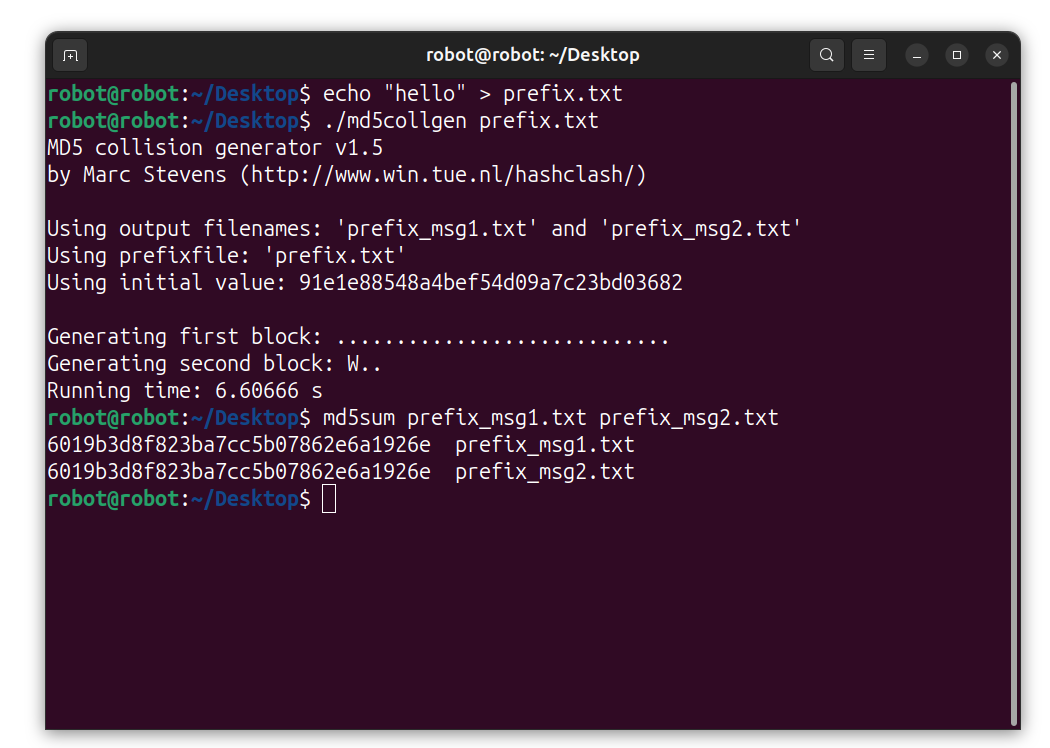
\includegraphics[width=0.9\linewidth]{image1.png}}
\caption{Running \texttt{md5collgen} (SEED Labs 2.0) with prefix \texttt{"hello"} on local Ubuntu.}
\label{fig:md5run}
\end{figure}

% --------------------------------
\subsection{Task 1 --- Question 3}
% --------------------------------

\textbf{Are the 128 bytes generated by md5collgen completely different for the two output files?}

No. The 128-byte collision block generated by \codebox{md5collgen} is \emph{partially} different --- only a handful of bytes differ, while the vast majority are identical. Figure~\ref{fig:diff} shows the byte-level diff from the VM.

\begin{figure}[H]
\centering
\fbox{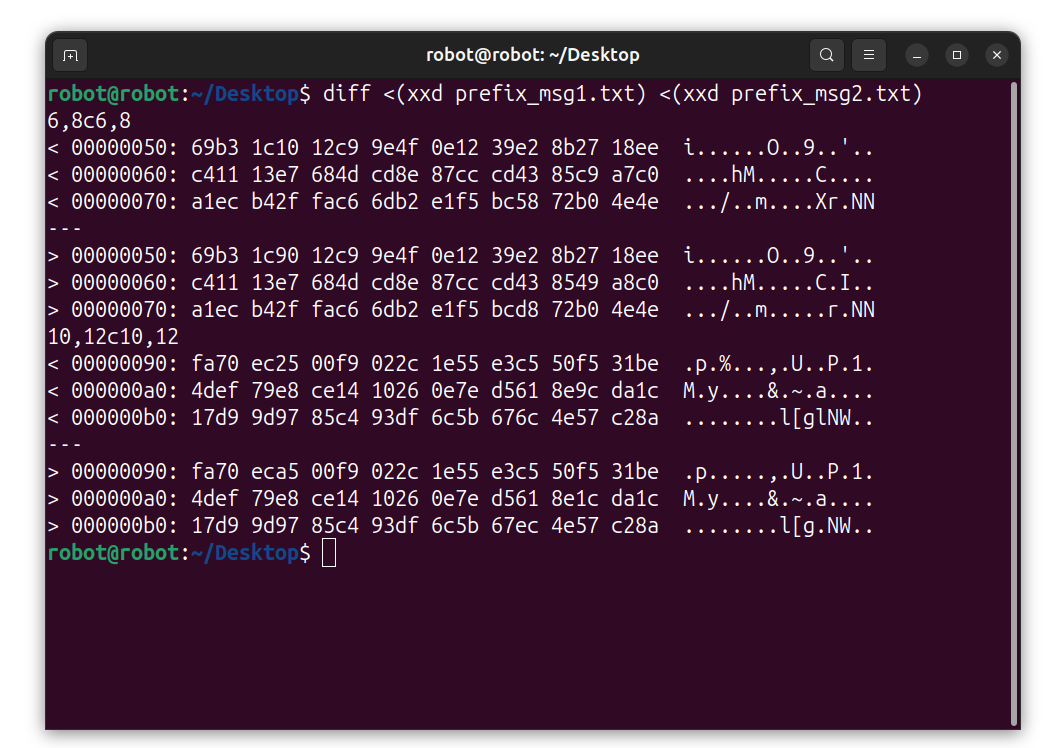
\includegraphics[width=0.9\linewidth]{image2.png}}
\caption{Hexdump diff between prefix\_msg1.txt and prefix\_msg2.txt --- differing bytes highlighted.}
\label{fig:diff}
\end{figure}

The two output files are each 192 bytes: a 64-byte padded prefix block followed by a 128-byte collision block. A byte-level comparison (Figure~\ref{fig:diff}) reveals that exactly \textbf{7 bytes} differ within the collision block (spanning bytes 64--191), while the remaining 121 bytes are identical:

\begin{table}[H]
\centering
\caption{Differing bytes between the two output files.}
\label{tab:diffbytes}
\footnotesize
\begin{tabular}{rccl}
\toprule
\textbf{Offset} & \textbf{msg1} & \textbf{msg2} & \textbf{Diff} \\
\midrule
83  & \texttt{0x10} & \texttt{0x90} & \texttt{+0x80} \\
109 & \texttt{0xc9} & \texttt{0x49} & \texttt{-0x80} \\
110 & \texttt{0xa7} & \texttt{0xa8} & \texttt{+0x01}$^\dag$ \\
123 & \texttt{0x58} & \texttt{0xd8} & \texttt{+0x80} \\
147 & \texttt{0x25} & \texttt{0xa5} & \texttt{+0x80} \\
173 & \texttt{0x9c} & \texttt{0x1c} & \texttt{-0x80} \\
187 & \texttt{0x6c} & \texttt{0xec} & \texttt{+0x80} \\
\bottomrule
\end{tabular}\\[3pt]
\footnotesize$^\dag$ Carry: \texttt{0xc9+0x80=0x149}, overflows byte~110 by~1.
\end{table}

Six of the seven changed bytes differ by exactly \codebox{0x80} (a single high-bit flip). The seventh byte (offset 110) changes by \codebox{+0x01} as an arithmetic carry: the 32-bit word at offsets 108--111 changes by \texttt{+0x8000}, which overflows byte 109 and propagates a carry into byte 110. The remaining 121 bytes of the collision block are byte-for-byte identical. Despite only these minor perturbations, both files produce the same MD5 hash \codebox{6019b3d8f823ba7cc5b07862e6a1926e}. This illustrates the Wang et al.\ differential attack underlying \codebox{md5collgen}: the tool engineers two 128-byte blocks whose difference cancels exactly through all four MD5 rounds, leaving both files with an identical final hash state.

% ============================================================
\section{Four-Party Diffie-Hellman Key Exchange}
% ============================================================

This section extends the 2-party DH protocol (Lab 4's \codebox{DH.py}) and the 3-party protocol (\codebox{DH3.py}) to four participants: \textbf{Alice}, \textbf{Bob}, \textbf{Carol}, and \textbf{Dave}. The goal is for all four to derive the same shared secret $K = g^{abcd} \bmod p$.

% --------------------------------
\subsection{Design: Extending 2-Party DH to Four Parties}
% --------------------------------

In the 2-party DH, Alice ($a$, $A=g^a$) and Bob ($b$, $B=g^b$) each raise the other's public key to their own private exponent: $K = B^a = A^b = g^{ab}$. The 3-party variant in \codebox{DH3.py} extends this with one extra round: a partial key $g^{ab}$ is relayed and raised to $c$, giving $g^{abc}$ for all three.

For four parties, a na{\"i}ve cyclic relay fails---each exponent would be applied more than once, yielding $g^{a^2b^2c^2d^2}$ instead of $g^{abcd}$. The correct approach is a \textbf{binary-tree} structure:

\begin{enumerate}[leftmargin=*, itemsep=0pt, topsep=2pt]
    \item \textbf{Round 1 (pairwise):} Pair (A,B) compute $K_{AB}=g^{ab}$; pair (C,D) compute $K_{CD}=g^{cd}$.
    \item \textbf{Round 2 (cross-exchange):} Each pair raises its partial key to both exponents of the other pair, obtaining $g^{abcd}$.
\end{enumerate}

Each private exponent appears exactly once in the final product, which is why the tree structure works where the cyclic relay does not.

% --------------------------------
\subsection{Protocol Description}
% --------------------------------

\textbf{Round 1 --- Pairwise DH.} Using the same $(g, p)$ parameters, each pair runs an independent 2-party DH:
\[
K_{AB} = B^a \bmod p = g^{ab}, \qquad K_{CD} = D^c \bmod p = g^{cd}
\]
Both partners in each pair independently verify they reach the same value (Alice checks $B^a$, Bob checks $A^b$, etc.).

\textbf{Round 2 --- Cross-exchange.} The two partial keys are raised to the remaining pair's private exponents:
\begin{align*}
\text{Alice \& Bob:}&\quad \bigl(K_{AB}^c\bigr)^d = (g^{ab})^{cd} = g^{abcd}\\
\text{Carol \& Dave:}&\quad \bigl(K_{CD}^a\bigr)^b = (g^{cd})^{ab} = g^{abcd}
\end{align*}

All four parties obtain the same value $K = g^{abcd}$. Since exponentiation is commutative in $\mathbb{Z}_p^*$, the order in which exponents are applied does not matter.

% --------------------------------
\subsection{Implementation}
% --------------------------------

The implementation (\codebox{DH4.py}) uses Python's \codebox{cryptography} library to generate a 1024-bit DH group $(g, p)$ and the four key pairs. The core computation is:

\begin{mycode}[Python]
# Round 1: pairwise DH
K_AB = pow(B, a, p)   # = g^(ab); Bob verifies: pow(A, b, p)
K_CD = pow(D, c, p)   # = g^(cd); Dave verifies: pow(C, d, p)

# Round 2: cross-exchange
K_alice = pow(pow(K_AB, c, p), d, p)  # (g^ab)^c^d = g^(abcd)
K_bob   = pow(pow(K_AB, c, p), d, p)
K_carol = pow(pow(K_CD, a, p), b, p)  # (g^cd)^a^b = g^(abcd)
K_dave  = pow(pow(K_CD, a, p), b, p)

assert K_alice == K_bob == K_carol == K_dave  # all match
\end{mycode}

The shared integer $K$ is converted to bytes and passed through \textbf{HKDF-SHA256} (32 bytes, \codebox{info=b'4party-DH-handshake'}) to produce an AES-256 key. Bob then encrypts a test message in AES-256-CBC mode; Alice decrypts it to confirm the shared key.

% --------------------------------
\subsection{Verification}
% --------------------------------

Running \codebox{python3 DH4.py} with freshly generated keys produces:

\begin{tcolorbox}[breakable, colback=gray!5, colframe=gray!50, arc=0pt, boxrule=0.5pt, left=5pt, right=5pt, top=5pt, bottom=5pt]
\begin{lstlisting}[language={}, basicstyle=\fontsize{7}{8}\ttfamily, breaklines=true, breakatwhitespace=false, columns=fixed]
=== Round 1: Pairwise DH ===
Alice computes K_AB = B^a mod p = g^(ab)
Bob   verifies K_AB = A^b mod p = g^(ab)  [OK]
Carol computes K_CD = D^c mod p = g^(cd)
Dave  verifies K_CD = C^d mod p = g^(cd)  [OK]

=== Round 2: Cross-Exchange ===
Alice: pow(pow(K_AB, c, p), d, p) = g^(abcd)
Bob:   pow(pow(K_AB, c, p), d, p) = g^(abcd)
Carol: pow(pow(K_CD, a, p), b, p) = g^(abcd)
Dave:  pow(pow(K_CD, a, p), b, p) = g^(abcd)

=== Verification ===
All four shared secrets match: True

Shared secret K = g^(abcd) (hex, 128 bytes):
376383894367af133fd477e900cdc4ba
79bdcfb0c56681dfbb368b9182265562
274a4d6c404b723f502a42aba98a622f
fd3275d871ab9c170e480f7697a135ce
6bd6fb098e188e6accec9bd18cca56f4
05c7438cced0ac758a2b3931b077a00c
1c4953e4d2a2dab8cf3fa29acb9bf346
ef455ad41856bb223d5e2e94105cc6a3

Derived AES-256 key (HKDF-SHA256, 32 bytes):
dcb542ab8ae86d0faadd43b948eb7c0f
29b9ed853b4b496eb608ab195925a34d

Plaintext  (Bob): b'Privacy Security|Bob -> Alice via 4-party DH!'
Ciphertext (AES-256-CBC, 48 bytes):
06ecf6d69506fafb6921f256a8f87b90
efd7f9f44df8b2a5596f65c0fab8a60a
eca5ce9e06d44309dea0109de816df98
IV: bacdd347b571487901152f790466d49d

Decrypted (Alice): b'Privacy Security|Bob -> Alice via 4-party DH!'
\end{lstlisting}
\end{tcolorbox}

The \codebox{assert} on line~56 of \codebox{DH4.py} passes without exception, confirming all four computed values are identical. Alice successfully decrypts Bob's ciphertext, providing end-to-end evidence that the shared secret $K = g^{abcd}$ was correctly established by all four parties.

% --------------------------------
\subsection{Security Considerations}
% --------------------------------

The binary-tree protocol inherits the security guarantees of 2-party DH. An eavesdropper who intercepts all public keys ($A, B, C, D$) and both intermediate values ($K_{AB} = g^{ab}$, $K_{CD} = g^{cd}$) still cannot compute $g^{abcd}$ without solving the \textbf{Computational Diffie-Hellman (CDH)} problem---believed to be as hard as the discrete logarithm in $\mathbb{Z}_p^*$. With a 1024-bit prime $p$, this is computationally infeasible for a passive adversary.

One limitation is that the protocol as simulated assumes a \emph{trusted broadcast channel}: in practice, each party would need to authenticate the intermediate values it receives (e.g., via digital signatures) to prevent man-in-the-middle attacks, in the same way that 2-party DH requires authenticated channels.

\end{document}
